\documentclass{template}
\usepackage{pdfpages}
\usepackage{setspace}
\usepackage{array}

\title{CSC 216 Portfolio 3}
\author{Nicolas Nytko}
\date{Dec 15, 2016}

\setcounter{tocdepth}{3}

\newcolumntype{L}{>{\arraybackslash}m{11cm}}

\begin{document}
\maketitle
\newpage
\tableofcontents
\newpage
\section{Paper}
\subsection{Perky Time Alotment {\footnotesize[sic]}}
Start with a background section to explain where PERT (Program Evaluation and Review Technique) came from. Next explain how PERT works and what it has to do with graphs and graph algorithms. Then expand to discuss how it is used today. Some suggestions are: construction, software development, etc. What does PERT have to do with CPM? What is CPM?

The following is a list of formatting requirements your paper(s) must follow:
 
\begin{itemize}
\item 2-5 pages:
  \begin{itemize}
  \item single spaced with 35\% (or less) of the 'body' space taken up by pictures/figures
  \item double spaced with no pictures/figures
  \item page count does NOT include a title page or list of references (both of which must be provided, however)
  \item page count does NOT include a table of contents nor an index (either of which may be provided, if you wish)
  \end{itemize}
\item margins:
    \begin{itemize}
    \item not more than 1.25 inches on a side
    \item not less than 0.5 inches on a side
    \end{itemize}
\item text fonts:
  \begin{itemize}
  \item something I can read!
  \item not less than 8 point
  \item not more than 12 point
  \end{itemize}
\item section/heading fonts:
  \begin{itemize}
  \item something I can read!
  \item not less than the text font
  \item not more than 4 more than the text font
  \end{itemize}
\item style:
  \begin{itemize}
  \item readable is preferred (spelling and grammar count!)
  \item must have an introduction, body, and conclusion
  \end{itemize}
\end{itemize}
\newpage
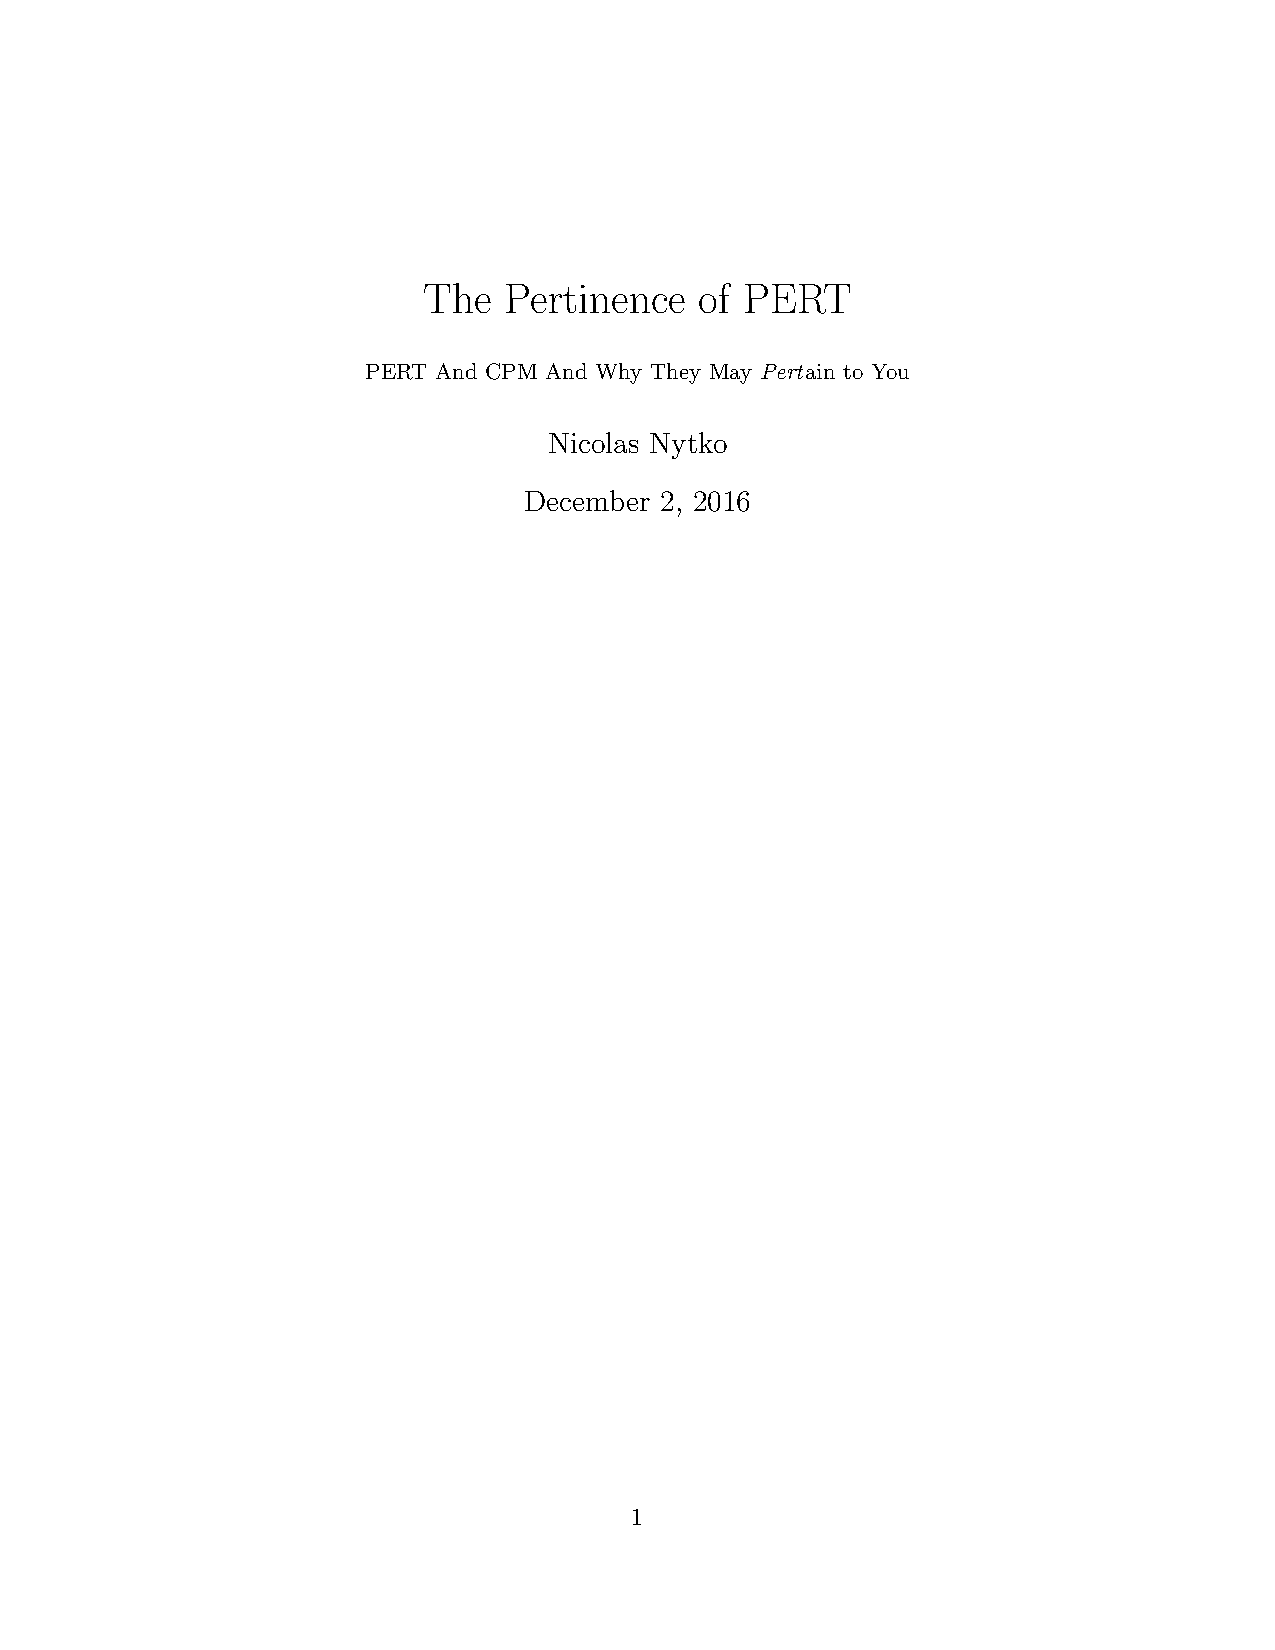
\includepdf[pages=-]{../paper/paper.pdf}
\section{Homework}
\subsection{Linked Lists}
\hwproblem{R-3.7}{
  Give an algorithm for finding the penultimate (second to last) node in a
  singly linked list where the last element is indicated by a null next link.
}
\srccode{../hw/r-3.7.cpp}
\hwproblem{R-3.10}{
  Describe a nonrecursive function for finding, by link hopping, the middle node
  of a doubly linked list with header and trailer sentinels. (Note: This
  function must only use link hopping; it cannot use a counter.) What is the
  running time of this function?
}
\srccode{../hw/r-3.10.cpp}
\hwproblem{C-3.3}{
  Let A be an array of size $n \geq 2$ containing integers from $1$ to $n - 1$,
  inclusive, with exactly one repeated. Describe a fast algorithm for finding
  the integer in A that is repeated.
}
\srccode{../hw/c-3.3.cpp}
\hwproblem{C-3.4}{
  Let B be an array of size $n \geq 6$ containing integers from $1$ to $n - 5$,
  inclusive, with exactly five repeated. Describe a good algorithm for finding
  the five integers in B that are repeated.
}

Sort B.  Create a variable that holds how many times the current value has been repeated, and a variable to hold what the last value was.
Loop through the array and increment the repeat variable every time the value has been repeated, and reset it to 0 when a new value is introduced.  End when the repeat value reaches 5.
\hwproblem{C-3.5}{
  Suppose you are designing a multi-player game that has $n \geq 1000$
  players, numbered $1$ to $n$, interacting in an enchanted forest. The winner of
  this game is the first player who can meet all the other players at least
  once (ties are allowed Assuming that there is a function meet(i, j), which is
  called each time a player i meets a player j (with $i \ne j$ ), describe
  a way to keep track of the pairs of meeting players and who is the winner.
}

Create a two dimensional boolean array with the x axis corresponding to the index of the player, and the y axis corresponding to whether that person was met.  So to see if player x has met player y, check array index \texttt{p[x][y]}.  If a full column is filled, then that player has met everyone.
\hwproblem{C-3.8}{
  Describe a good algorithm for concatenating two singly linked lists L and M,
  with header sentinels, into a single list L' that contains all the nodes of L
  followed by all the nodes of M. Create a new list L' and copy all of the nodes
  from L into it. At the end of L', copy all of the nodes of M.
}

Copy all of the elements from L into L'.  Start copying M at the last node of L' after the header sentinel and continue until the null pointer.
\hwproblem{C-3.9}{
  Give a fast algorithm for concatenating two doubly linked lists L and M, with
  header and trailer sentinel nodes, into a single list L′.
}
Remove L's trailing sentinel and M's header sentinel and save L's last node and M's first node, we will call them L' and M' respectively.  Set L' next to M', the previous of M' to L.  The lists are now concatenated.
Copy all the nodes from L into L'.  Copy the nodes from M into the end of L'.  Set the next 
\hwproblem{C-3.10}{
  Describe in detail how to swap two nodes x and y (and not just their contents)
  in a singly linked list L given references only to x and y. Repeat this
  exercise for the case when L is a doubly linked list. Which algorithm takes
  more time?
}

For a singly linked list: loop through until the nodes before x and y are found, label them x' and y'.  Set x' next node to y, and y next to x original next.  Set y' next node to x, and x next node to y original next.

For a doubly linked list: do the same thing except time is not needed to loop through and find the previous nodes.  Don't forget to set the previous node values.
\hwproblem{C-3.11}{
  Describe in detail an algorithm for reversing a singly linked list L using
  only a constant amount of additional space and not using any recursion.
}
Define n to be the size of the linked list.  Loop \texttt{n-1} times with iterator i starting at 0, and bring node \texttt{n-i} backwards by swapping it \texttt{n-i} times with the node previous.  Save the previous node as a pointer variable.

\hwproblem{C-3.22}{
  Suppose you are given two circularly linked lists, L and M, that is, two lists
  of nodes such that each node has a nonnull next node. Describe a fast
  algorithm for telling if L and M are really the same list of nodes but with
  different (cursor) starting points.
}

Create two node pointers, lowercase l and m, and set them to point to the head of L and M respectively.  Loop through the list until l is equal to M and m is equal to L (they are the same list), or l is equal to L and m is equal to M (the whole list has been parsed and L and M are not the same list).

\hwproblem{C-3.23}{
  Given a circularly linked list L containing an even number of nodes,
  describe how to split L into two circularly linked lists of half the size.
}

Given a circularly linked list L, define M to be the length of L divided by two.
Create two node pointers, x and y, and have them point to the beginning of L and the node at M, respectively.  For the last node in the first half (M-1), set its next node to the first node.  For the first node in the first half (0), set its previous node to M-1.  For node M, set its previous node to the last node in the list.  Set the last node's next to M.
\newpage
\section{Labs}
\subsection{Bucket Sort}
\info{Bucket Sort}{2}{
  Design and implement a version of the bucket-sort algorithm for sorting a linked list of $n$ entries (for instance, a list of type \texttt{std::list<int>}) with integer keys taken from the range $[0, N − 1]$, for $N \geq 2$. The algorithm should run in $O(n + N)$ time.
}
\subsubsection{Compiler Environment}
\srcfile{environment}
\subsubsection{Source}
\srccode{../lab/bucketsort/main.cpp}
\subsubsection{Compiler Output}
\srcfile{../lab/bucketsort/compilerout}
\subsubsection{Program Output}
\srcfile{../lab/bucketsort/progout}
\subsection{Leprechaun Simulator}
\info{Jumping Leprechauns}{3}{
  Write a program that performs a simple n-body simulation, called “Jumping Leprechauns.” This simulation involves n leprechauns, numbered $1$ to $n$. It maintains a gold value $g_i$ for each leprechaun $i$, which begins with each leprechaun starting out with a million dollars worth of gold, that is, $g_i = 1000000$ for each $i = 1,2,\ldots,n$. In addition, the simulation also maintains, for each leprechaun, $i$, a place on the horizon, which is represented as a double-precision floating point number, $x_i$. In each iteration of the simulation, the simulation processes the leprechauns in order. Processing a leprechaun $i$ during this iteration begins by computing a new place on the horizon for $i$, which is determined by the assignment
\[x_i\leftarrow x_i+rg_i\]
where $r$ is a random floating-point number between $−1$ and $1$. The leprechaun $i$ then steals half the gold from the nearest leprechauns on either side of him and adds this gold to his gold value, $g_i$. Write a program that can perform a series of iterations in this simulation for a given number, $n$, of leprechauns. You must maintain the set of horizon positions using an ordered map data structure described in this chapter.
}
\subsubsection{Compiler Environment}
\srcfile{environment}
\subsubsection{Source}
\srccode{../lab/leprechaun/main.cpp}
\srccode{../lab/leprechaun/btree.hpp}
\srccode{../lab/leprechaun/orderedmap.hpp}
\subsubsection{Compiler Output}
\srcfile{../lab/leprechaun/compilerout}
\subsubsection{Program Output}
\srcfile{../lab/leprechaun/progout}

\end{document}